\section{Requisiti soddisfatti}

\subsection{Tabella del soddisfacimento dei requisiti}

\begin{longtable}{C{3cm} C{3cm} L{5.5cm} C{3cm}}
\rowcolor{white}\caption{Tabella del soddisfacimento dei requisiti}\\
		\rowcolor{redafk}
\textcolor{white}{\textbf{Codice}} & \textcolor{white}{\textbf{Esito}}\\
		\endfirsthead
		\rowcolor{white}\caption[]{(continua)} \\
		\rowcolor{redafk}
\textcolor{white}{\textbf{Codice}} & \textcolor{white}{\textbf{Esito}}\\
		\endhead
		
Re1F1 	& Soddisfatto\\
Re1F1.1 & Soddisfatto\\
Re1F1.2 & Soddisfatto\\
Re1F1.3 & Soddisfatto\\
Re2F1.4 & Soddisfatto\\
Re2F1.5 & Soddisfatto\\
Re1F1.6 & Soddisfatto\\
Re1F2 	& Soddisfatto\\
Re1F2.1 & Soddisfatto\\
Re1F2.2 & Soddisfatto\\
Re2F2.3 & Soddisfatto\\
Re1F2.4 & Soddisfatto\\
Re1F3 	& Non soddisfatto\\
Re1F3.1 & Soddisfatto\\
Re1F3.2 & Soddisfatto\\
Re3F3.3 & Non soddisfatto\\ 
Re1F3.4 & Soddisfatto\\
Re2F3.5 & Non soddisfatto\\
Re1F3.6 & Soddisfatto\\
Re1F4 	& Soddisfatto\\
Re1F4.1 & Soddisfatto\\
Re1F4.2 & Soddisfatto\\
Re1F4.3 & Soddisfatto\\
Re2F4.4 & Soddisfatto\\
Re1F4.5 & Soddisfatto\\
Re1F5 	& Non soddisfatto\\
Re1F5.1 & Soddisfatto\\
Re1F5.2 & Non soddisfatto\\
Re2F5.3 & Soddisfatto\\
Re1F5.4 & Non soddisfatto\\
Re2F5.5 & Non soddisfatto\\
Re1F5.6 & Non soddisfatto\\
Re1F6 	& Soddisfatto\\
Re1F6.1 & Soddisfatto\\
Re3F6.2 & Non soddisfatto\\
Re1F7 	& Soddisfatto\\
Re1F8 	& Soddisfatto\\
Re1F9 	& Soddisfatto\\
Re1F10 	& Non soddisfatto\\
Re1F11 	& Non soddisfatto\\
Re1F12 	& Non soddisfatto\\
Re1F13 	& Non soddisfatto\\
Re1F14 	& Non soddisfatto\\
Re1Q1 	& Soddisfatto\\
Re1Q2 	& Soddisfatto\\
Re1Q2.1 & Soddisfatto\\
Re2Q2.2 & Non soddisfatto\\
Re1Q3 	& Soddisfatto\\
Re1Q4 	& Soddisfatto\\
Re2Q5 	& Soddisfatto\\
Re2Q6 	& Soddisfatto\\
Re2Q7 	& Soddisfatto\\
Re1V1 	& Soddisfatto\\
Re1V1.1 & Soddisfatto\\
Re1V1.2 & Soddisfatto\\
Re1V1.3 & Soddisfatto\\
Re1V1.4 & Soddisfatto\\
Re1V2 	& Soddisfatto\\
Re1V3 	& Soddisfatto\\
Re1V4 	& Soddisfatto\\
Re1V5 	& Soddisfatto\\
\end{longtable}

\subsection{Grafici del soddisfacimento dei requisiti}
Dei 61 requisiti individuati, 46 sono stati stati soddisfatti, risultando quindi in una copertura del 75\%.\\
\begin{figure}[H]
\centering
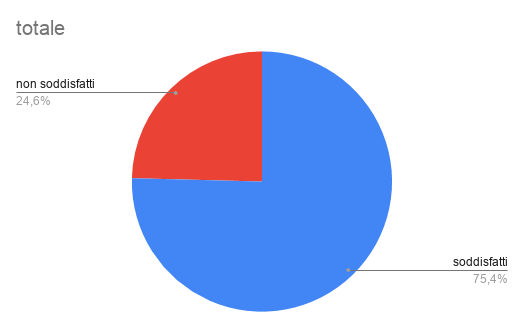
\includegraphics[scale=0.75]{img/grafici/totale.png}
\caption{Totale requisiti soddisfatti}
\end{figure}

I requisiti obbligatori sono 48 sui 61 totali. Di questi 48 requisiti 38 sono stati soddisfatti completamente, risultando in una copertura del 79\%; i restanti 10 requisiti sono messaggi d'errore o d'avviso che non sono quindi necessari al corretto funzionamento del prodotto. Alcuni di questi requisiti sono però già presenti in una implementazione parziale.
\begin{figure}[H]
\centering
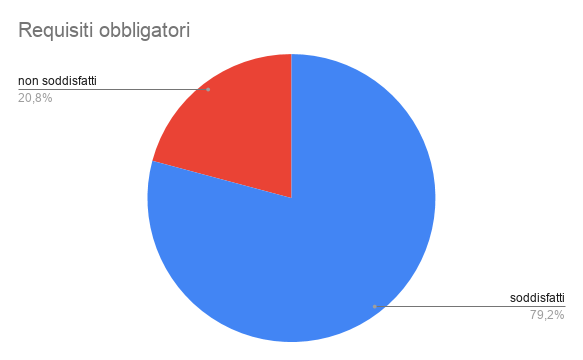
\includegraphics[scale=0.75]{img/grafici/Requisiti_obbligatori.png}
\caption{Requisiti obbligatori soddisfatti}
\end{figure}

I requisiti desiderabili e opzionali sono 13 sui 61 totali. di questi 13 requisiti 8 sono stati soddisfatti completamente, risultando quindi in una copertura del 61\%.
\begin{figure}[H]
\centering
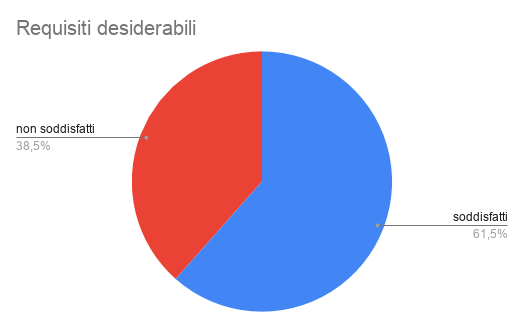
\includegraphics[scale=0.75]{img/grafici/Requisiti_desiderabili.png}
\caption{Requisiti desiderabili e opzionali soddisfatti}
\end{figure}